\section{Creation of DeepFakes}\label{sect:creation-of-deepfakes}
Statistical models come in multiple classes with divergent properties.
One such discrimination is that between discriminative and generative models.
Generative models learn the statistical properties of the input domain~\cite[cf.][\nopp~651\psqq]{Goodfellow.2016}.
For example, they are able to generate unique images of human faces, based on
previously observed ones~\cite{Karras.2019}. 

\par
Generative models are thus the focus of techniques for creating DeepFakes.
For an introduction to the creation of DeepFakes, the scope is limited to
\glspl{rnn}, \glspl{ae} and \glspl{gan}.
\begin{figure}[h]
    \center{}
    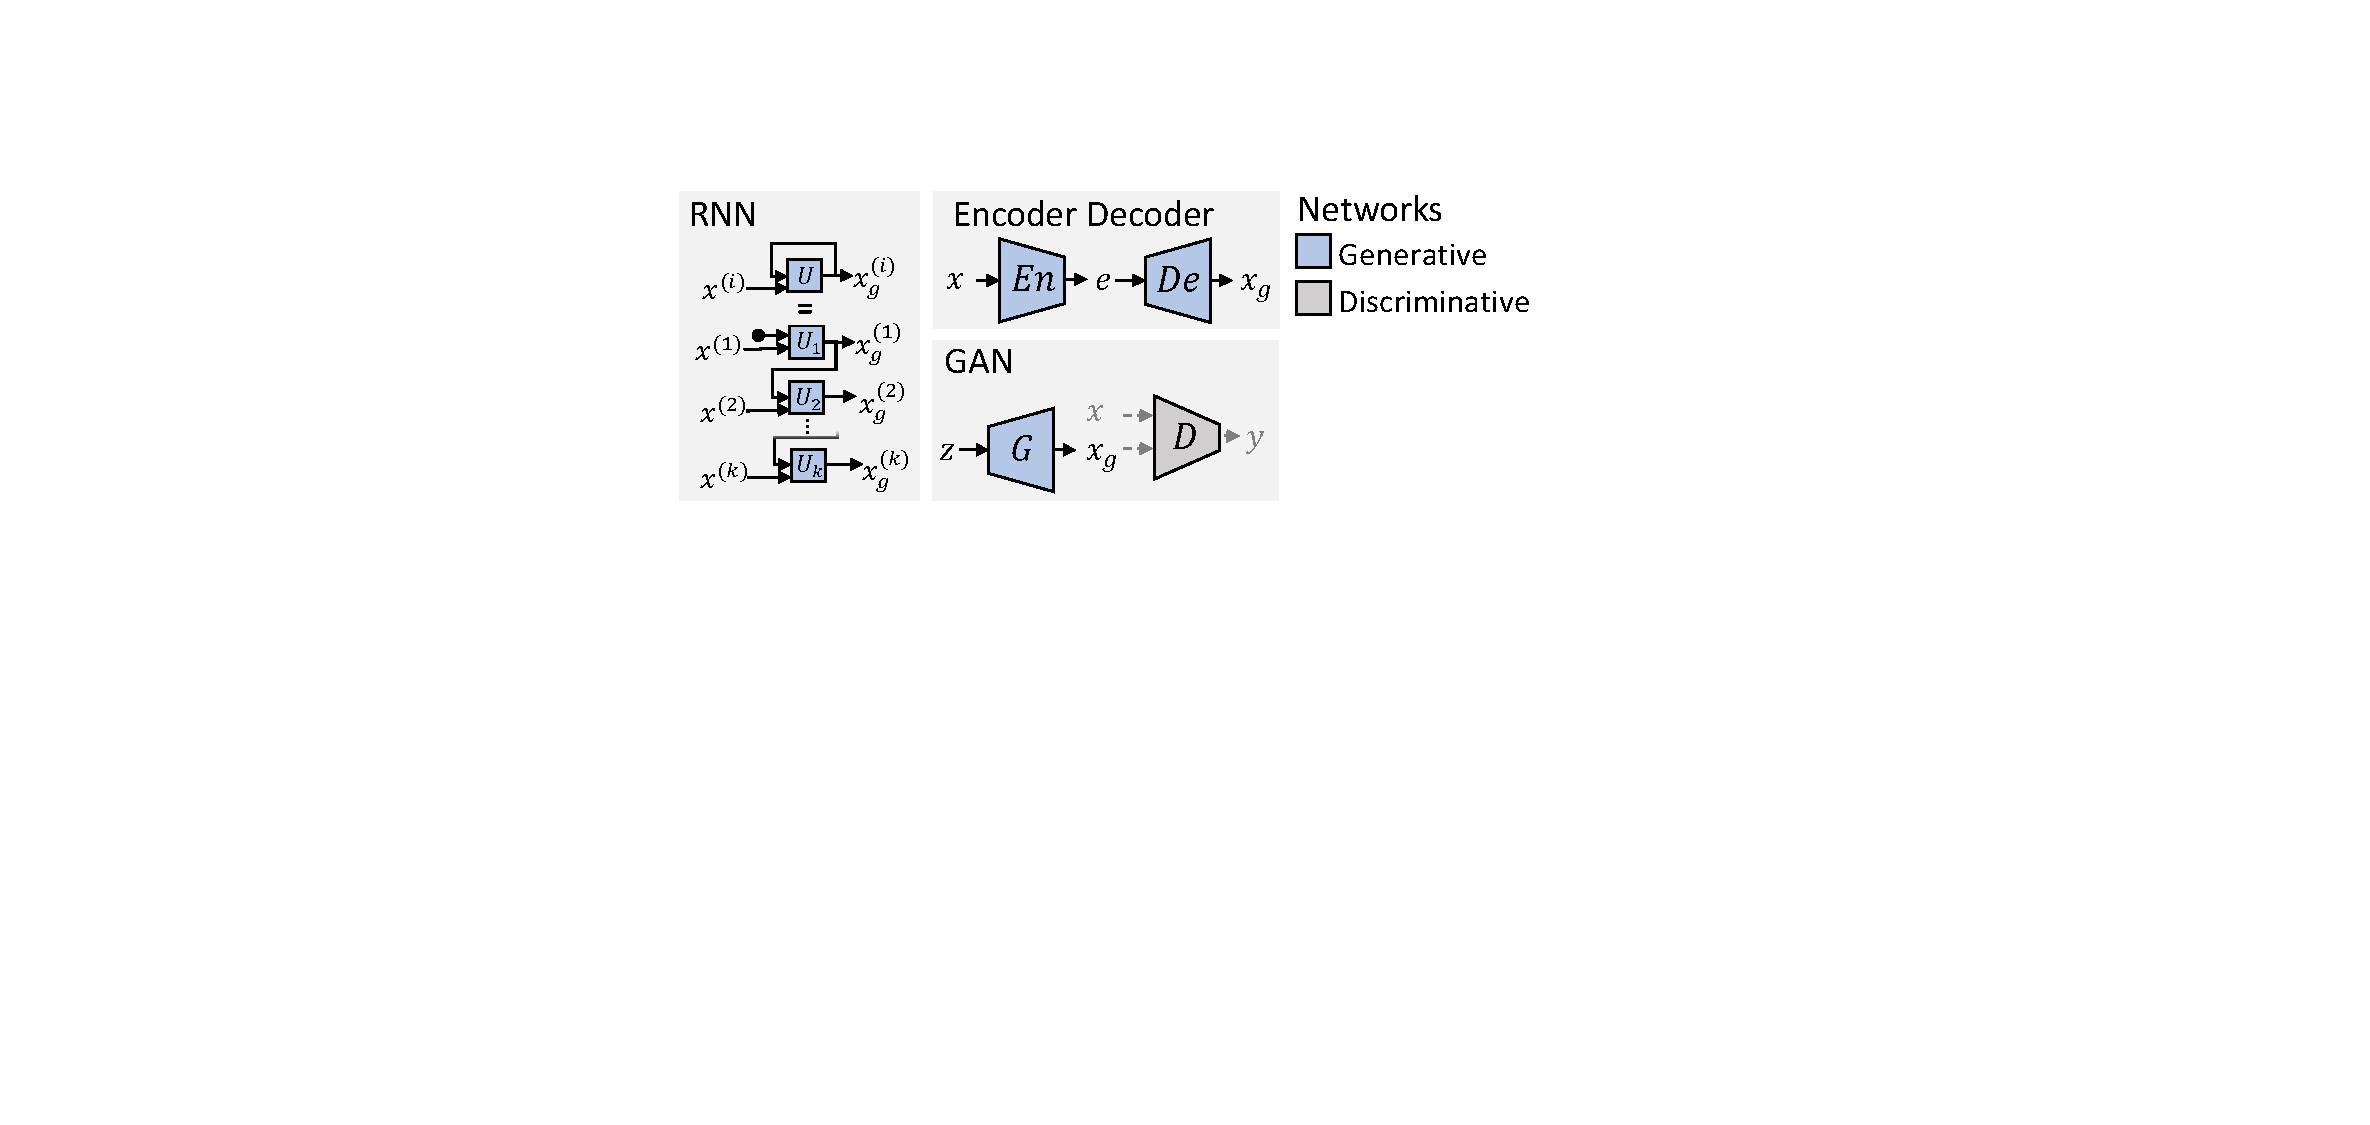
\includegraphics[width=0.65\textwidth]{basic_nns2.pdf}
    \caption{Selection of generative models, adopted from~\cite{Mirsky.2020}}\label{fig:drain-parse-tree}
\end{figure}
